\documentclass{article}
\usepackage[utf8]{inputenc}
\usepackage{vmargin}


\usepackage{amsmath} 
\usepackage{graphicx}
\usepackage{graphics}
\usepackage{float}
\usepackage{blindtext}
\usepackage{listings}
\usepackage{xcolor}
\usepackage[spanish]{babel}
\usepackage{subfig}

\graphicspath{ {images/} }
\title{Operador Logarítmico}
\date{}
\setpapersize{A4}
\setmargins{2.5cm}       % margen izquierdo
{1.5cm}                        % margen superior
{16.5cm}                      % anchura del texto
{23.42cm}                    % altura del texto
{10pt}                           % altura de los encabezados
{1cm}                           % espacio entre el texto y los encabezados
{0pt}                             % altura del pie de página
{2cm}                           % espacio entre el texto y el pie de página

\begin{document}

%-------COLORES PARA CODIGO ------------------------
\lstdefinestyle{customc}{
  belowcaptionskip=1\baselineskip,
  breaklines=true,
  frame=L,
  xleftmargin=\parindent,
  language=JavaScript,
   basicstyle=\footnotesize\ttfamily,
  showstringspaces=false,
  basicstyle=\footnotesize\ttfamily,
  keywordstyle=\bfseries\color{green!40!black},
  commentstyle=\itshape\color{purple!40!black},
  identifierstyle=\color{blue},
  stringstyle=\color{orange},
  frame=single,	  
  numbers=left,
   numberstyle=\footnotesize,
}

\lstdefinestyle{customasm}{
  belowcaptionskip=1\baselineskip,
  frame=L,
  xleftmargin=\parindent,
  language=JavaScript,
  basicstyle=\footnotesize\ttfamily,
  commentstyle=\itshape\color{purple!40!black},
}

\lstset{escapechar=@,style=customc}

%---------------------------------------------

\thispagestyle{empty}

\vfill
 \begin{center}
    \begin{figure}[h]
    \centering
    \includegraphics[width=12cm]{unsa}\\
    
    \end{figure}
 	 
     \vspace*{1.5cm}
    {\large\bfseries FACULTAD DE PRODUCCIÓN Y SERVICIOS} \\
    {\large\bfseries ESCUELA PROFESIONAL DE CIENCIA DE LA COMPUTACIÓN}  \\    
    \vspace*{1.5cm}
    
 	\rule[0.5ex]{\linewidth}{2pt}\vspace*{-\baselineskip}\vspace*		{3.2pt}
	\rule[0.5ex]{\linewidth}{1pt}\\[\baselineskip]
 	{\huge Física Computacional} \\[4mm]
    \rule[0.5ex]{\linewidth}{1pt}\vspace*{-							\baselineskip}\vspace{3.2pt}
	\rule[0.5ex]{\linewidth}{2pt}\\
 	\vspace*{1cm}

    \begin{large} \bfseries
    Tarea leyes de Newton \\
    
    \vspace{5mm}
    Eduardo Antonio Sánchez Hincho \\

    \vspace{5mm}
    Docente:\\
    Edwin Agapito Llamoca Requena
    \end{large}
    \vspace*{0.4in}
    
    \noindent \\
    
    \vfill
    \large\bfseries{ AREQUIPA\\2020}
\end{center}
\newpage
\section{Movimiento circular}
Para los siguientes ejercicios, el código fue el mismo, solo se variaron ciertas cosas.
\subsection{1}
\begin{lstlisting}[language=Python,caption=Desafío 1.1]
import matplotlib.pyplot as plt
import numpy as np
from mpl_toolkits.mplot3d import Axes3D

h = 0.00001
r=8
m=5
pos = [[r],[0],[0]]
velocidad = [[0],[4],[0]]
a = [-2,0]
tiempo = 20
pt = np.arange(0, tiempo, h)

for i in pt:
    x = pos[0][-1]
    y = pos[1][-1]

    pos[0].append(x + velocidad[0][-1]*h)
    pos[1].append(y + velocidad[1][-1]*h)

    a = [-2 * x/r, -2 * y/r]

    velocidad[0].append(velocidad[0][-1] + a[0]*h)
    velocidad[1].append(velocidad[1][-1] + a[1]*h)

plt.xlim(-r-1,r+1)
plt.ylim(-r-1,r+1)
plt.plot(pos[0],pos[1])    
plt.xlabel('espacio-x')
plt.ylabel('espacio-y')
plt.title('y-x')
plt.grid(True)

plt.show()
\end{lstlisting}
\begin{figure}[H]
    \centering
    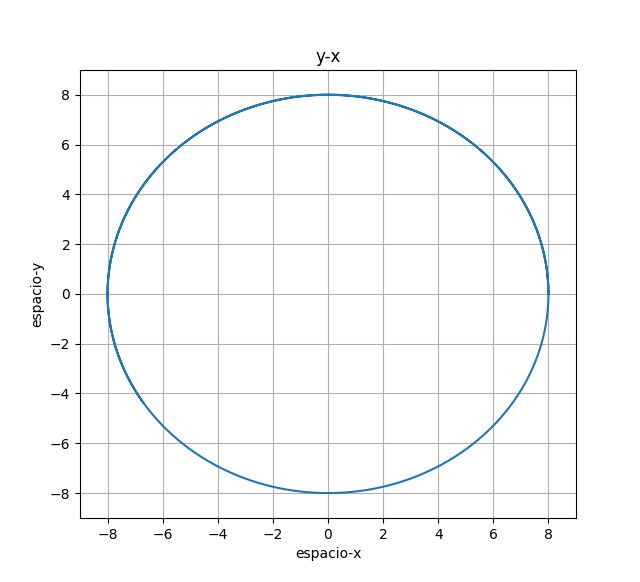
\includegraphics[width=0.5\textwidth]{1.png}
    \caption{Resultado}
\end{figure}

\subsection{2}
El código vario en lo siguiente
\begin{lstlisting}[language=Python,caption=Desafío 1.1]
pos = [[0],[r],[0]]
velocidad = [[-4],[0],[0]]
a = [0,-2]
\end{lstlisting}
El resultado fue el mismo que el anterior.
\begin{figure}[H]
    \centering
    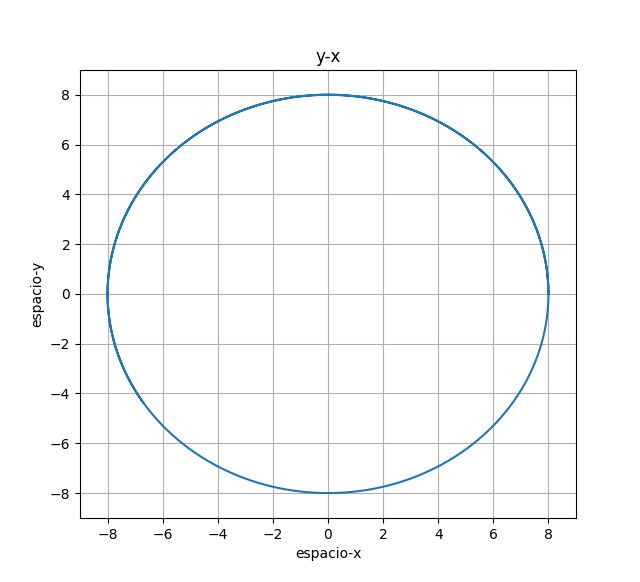
\includegraphics[width=0.5\textwidth]{1.png}
    \caption{Resultado}
\end{figure}
\subsection{3}
\begin{lstlisting}[language=Python,caption=Desafío 1.1]
pos = [[-r],[0],[0]]
velocidad = [[0],[-4],[0]]
a = [2,0]
\end{lstlisting}

\subsection{4}
\begin{lstlisting}[language=Python,caption=Desafío 1.1]
pos = [[0],[-r],[0]]
velocidad = [[4],[0],[0]]
a = [0,2]
\end{lstlisting}

\subsection{5}
\begin{lstlisting}[language=Python,caption=Desafío 1.1]
pos = [[0],[-r],[0]]
velocidad = [[4],[0],[0]]
ac = 2
a = [-ac*np.cos(np.pi/4),-ac*np.sin(np.pi/4)]
\end{lstlisting}
Para todos estos, obtuvimos el mismo círculo
\begin{figure}[H]
    \centering
    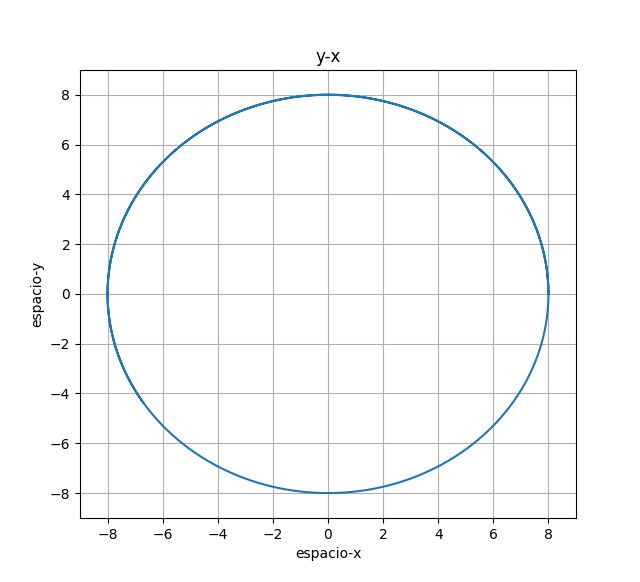
\includegraphics[width=0.5\textwidth]{1.png}
    \caption{Resultado}
\end{figure}

\subsection{6}
Se aplico la formula de Euler para hallar la velocidad en todos los tiempos.
\begin{lstlisting}[language=Python,caption=Desafío 1.1]
import matplotlib.pyplot as plt
import numpy as np
import math

h = 0.001
r=8
m=5
pos = [[0],[-r],[0]]
velocidad = [[4],[0],[0]]
a = [0,2]
tiempo = 20
pt = np.arange(0, tiempo, h)

for i in pt:
    x = pos[0][-1]
    y = pos[1][-1]

    pos[0].append(x + velocidad[0][-1]*h)
    pos[1].append(y + velocidad[1][-1]*h)

    vx = velocidad[0][-1]
    vy = velocidad[1][-1]

    print("velocidad x = ",vx, " , ", "velocidad y = ", vy, "=", end ="" )
    print(math.sqrt(pow(vx,2)+pow(vy,2)), end = "\n")

    a = [-2 * x/r, -2 * y/r]

    velocidad[0].append(velocidad[0][-1] + a[0]*h)
    velocidad[1].append(velocidad[1][-1] + a[1]*h)
\end{lstlisting}
El resultado siempre fue un número aproximado a 4
\begin{figure}[H]
    \centering
    \includegraphics[width=1\textwidth]{6.png}
    \caption{Resultado}
\end{figure}

\subsection{7}
\begin{lstlisting}[language=Python,caption=Desafío 1.1]
h = 0.001
r=8
m=5
pos = [[0],[-r],[0]]
velocidad = [[4],[0],[0]]
a = [0,2]
ac = 2
tiempo = 20
pt = np.arange(0, tiempo, h)

for i in pt:
    x = pos[0][-1]
    y = pos[1][-1]

    pos[0].append(x + velocidad[0][-1]*h)
    pos[1].append(y + velocidad[1][-1]*h)

    vx = velocidad[0][-1]
    vy = velocidad[1][-1]

    print("Fuerza centripeta en", i, end =" = " )
    print(m*ac, end = "\n")

    a = [-2 * x/r, -2 * y/r]

    velocidad[0].append(velocidad[0][-1] + a[0]*h)
    velocidad[1].append(velocidad[1][-1] + a[1]*h)
\end{lstlisting}
El resultado en todos los tiempos, siempre fue 10
\begin{figure}[H]
    \centering
    \includegraphics[width=0.5\textwidth]{7.png}
    \caption{Resultado}
\end{figure}
\subsection{8}
\begin{center}
    $\displaystyle \frac{L}{T^2}= L^x \frac{L^y}{T^y}$ \\
    \vspace*{0.3 cm}
    $L.T^-^2 = L^X^+^Y . T^-^y$\\
    \vspace*{0.3 cm}
    $x+y=1$ \\
    \vspace*{0.3 cm}
    $-y=-2$ \\ $y=2$\\
    \vspace*{0.3 cm}
    $x+2=1$ \\ $x=-1$
\end{center}

\subsection{9}
\begin{center}
     $L.T^-^2= v^2/r = a_c$ \\
\end{center}
Si ejecutamos la formula en cada instruccion, tendremos lo siguiente.
\begin{lstlisting}[language=Python,caption=Desafío 1.1]
v = 50
angulo = np.deg2rad(60)
C = 0.5
m = 0.145
r = 0.0367
A = np.pi * r * r
p = 1.2

h = 0.001
pos = [[0],[0]]
k = (1/2) * (C*A*p/m)
velocidad = [[v*np.cos(angulo)], [v*np.sin(angulo)]]
a = [-k*v*velocidad[0][0], -10-k*v*velocidad[1][0]]

pos2 = [[0],[0]]
k2 = 0
velocidad2 = [[v*np.cos(angulo)], [v*np.sin(angulo)]]
a2 = [-k2*v*velocidad2[0][0], -10-k2*v*velocidad2[1][0]]

print(np.sin(angulo))
while True:
    pos2[0].append(pos2[0][-1] + velocidad2[0][-1]*h)
    pos2[1].append(pos2[1][-1] + velocidad2[1][-1]*h)

    velocidad2[0].append(velocidad2[0][-1] + a2[0]*h)
    velocidad2[1].append(velocidad2[1][-1] + a2[1]*h)

    if(pos[1][-1] >= 0):
        pos[0].append(pos[0][-1] + velocidad[0][-1]*h)
        pos[1].append(pos[1][-1] + velocidad[1][-1]*h)

        velocidad[0].append(velocidad[0][-1] + a[0]*h)
        velocidad[1].append(velocidad[1][-1] + a[1]*h)

        v = math.sqrt(pow(velocidad[0][-1],2) + pow(velocidad[1][-1],2))
        a[0] = -k * v * velocidad[0][-1]
        a[1] = -10 -k * v * velocidad[1][-1]

    if(pos[1][-1] < 0):
        break
\end{lstlisting}
El resutlado fue
\begin{figure}[H]
    \centering
    \includegraphics[width=0.5\textwidth]{9.png}
    \caption{Resultado}
\end{figure}
Como vemos, obtuvimos un resultado cercano a 2 en todos los casos.

\section{Movimiento de proyectiles cuando se presenta la resistencia
del aire}

Se realizó lo siguiente
\begin{lstlisting}[language=Python,caption=Desafío 1.1]
v = 50
angulo = np.deg2rad(60)
C = 0.5
m = 0.145
r = 0.0367
A = np.pi * r * r
p = 1.2

h = 0.001
pos = [[0],[0]]
k = (1/2) * (C*A*p/m)
velocidad = [[v*np.cos(angulo)], [v*np.sin(angulo)]]
a = [-k*v*velocidad[0][0], -10-k*v*velocidad[1][0]]

pos2 = [[0],[0]]
k2 = 0
velocidad2 = [[v*np.cos(angulo)], [v*np.sin(angulo)]]
a2 = [-k2*v*velocidad2[0][0], -10-k2*v*velocidad2[1][0]]

print(np.sin(angulo))
while True:
    pos2[0].append(pos2[0][-1] + velocidad2[0][-1]*h)
    pos2[1].append(pos2[1][-1] + velocidad2[1][-1]*h)

    velocidad2[0].append(velocidad2[0][-1] + a2[0]*h)
    velocidad2[1].append(velocidad2[1][-1] + a2[1]*h)

    if(pos[1][-1] >= 0):
        pos[0].append(pos[0][-1] + velocidad[0][-1]*h)
        pos[1].append(pos[1][-1] + velocidad[1][-1]*h)

        velocidad[0].append(velocidad[0][-1] + a[0]*h)
        velocidad[1].append(velocidad[1][-1] + a[1]*h)

        v = math.sqrt(pow(velocidad[0][-1],2) + pow(velocidad[1][-1],2))
        a[0] = -k * v * velocidad[0][-1]
        a[1] = -10 -k * v * velocidad[1][-1]

    if(pos[1][-1] < 0):
        break
\end{lstlisting}
El resultado individual con fuerza de arrastre es:
\begin{figure}[H]
    \centering
    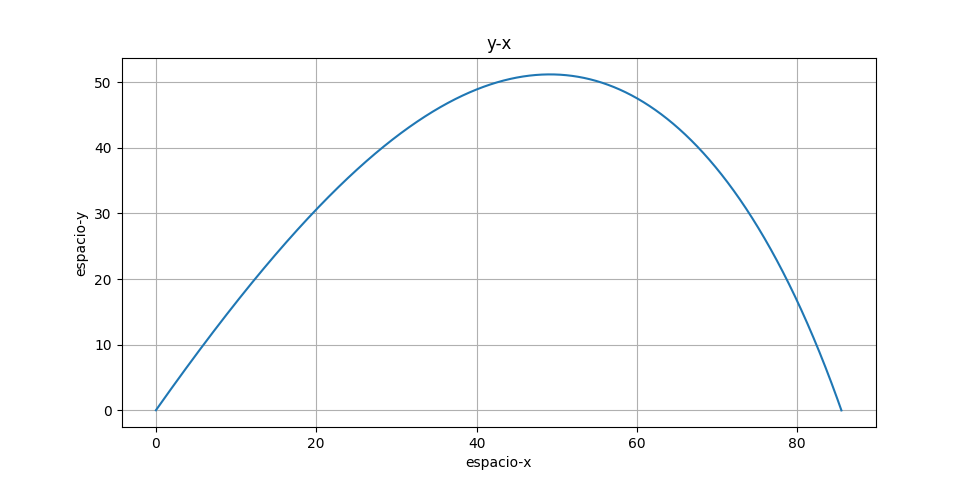
\includegraphics[width=1\textwidth]{2_2.png}
    \caption{Resultado}
\end{figure}
El resultado sin fuerza de arrastre, junto al anterior es:
\begin{figure}[H]
    \centering
    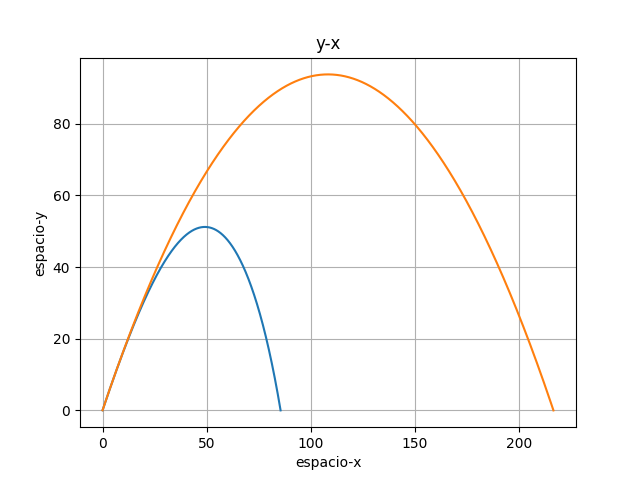
\includegraphics[width=1\textwidth]{2_1.png}
    \caption{Resultado}
\end{figure}
Se puede observar la gran diferencia de resultados.

\section{Desafío}
Se implemento lo siguiente para el problema dapo.
\begin{lstlisting}[language=Python,caption=Desafío 1.1]
import matplotlib.pyplot as plt
import numpy as np
import math
from mpl_toolkits.mplot3d import Axes3D

r=0.005
vl = 4/3*np.pi*r**3
C = 0.5
d = 1000
m = d*vl
r = 0.0367
A = np.pi*r**2
p = 1.2

h = 0.001
pos = [[0],[16]]
k = (1/2) * (C*A*p/m)
velocidad = [[14], [0]]
a = [0, -10]

while True:
    pos[0].append(pos[0][-1] + velocidad[0][-1]*h)
    pos[1].append(pos[1][-1] + velocidad[1][-1]*h)

    velocidad[0].append(velocidad[0][-1] + a[0]*h)
    velocidad[1].append(velocidad[1][-1] + a[1]*h)

    v = math.sqrt(pow(velocidad[0][-1],2) + pow(velocidad[1][-1],2))
    a[0] = -k * v * velocidad[0][-1]
    a[1] = -10 -k * v * velocidad[1][-1]

    if(pos[1][-1] < 0):
        break

plt.plot(pos[0],pos[1])
plt.xlabel('espacio-x')
plt.ylabel('espacio-y')
plt.title('y-x')
plt.grid(True)

plt.show()
\end{lstlisting}
Los resultados fueron los siguientes
\begin{figure}[H]
    \centering
    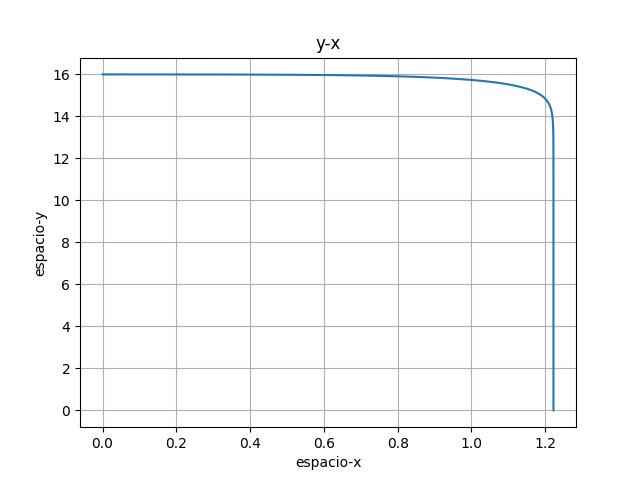
\includegraphics[width=1\textwidth]{3_1.png}
    \caption{Resultado}
\end{figure}

\section{Cálculo de los errores para el ejercicio de movimiento circular}
Se hizo el siguiente código para calcular el error después de una vuelta
\begin{lstlisting}[language=Python,caption=Desafío 1.1]
h = 0.1
r=8
m=5
pos = [[r],[0],[0]]
velocidad = [[0],[4],[0]]
a = [-2,0]
tiempo = 12.6
pt = np.arange(0, tiempo, h)

for i in pt:
    x = pos[0][-1]
    y = pos[1][-1]

    pos[0].append(x + velocidad[0][-1]*h)
    pos[1].append(y + velocidad[1][-1]*h)

    a = [-2 * x/r, -2 * y/r]

    velocidad[0].append(velocidad[0][-1] + a[0]*h)
    velocidad[1].append(velocidad[1][-1] + a[1]*h)

rsimulado = np.sqrt(pow(pos[0][-1],2)+pow(pos[1][-1],2))

error = np.abs(rsimulado - r)/r*100

print(f'El error con un h de {h} despues de una vuelta es {error}')
\end{lstlisting}
Se probo con varios valores de h
\begin{figure}[H]
    \centering
    \includegraphics[width=1\textwidth]{4_1.png}
    \caption{Resultado}
\end{figure}
Como vemos, a menor valor de h, menor error.

\end{document}


